% options:
% thesis=B bachelor's thesis
% thesis=M master's thesis
% czech thesis in Czech language
% english thesis in English language

\documentclass[thesis=M,czech]{FITthesis}[2011/07/15]

\usepackage[utf8]{inputenc} % LaTeX source encoded as UTF-8
\usepackage{eurosym}
\usepackage{float}
\usepackage{graphicx} %graphics files inclusion
% \usepackage{subfig} %subfigures
% \usepackage{amsmath} %advanced maths
% \usepackage{amssymb} %additional math symbols

% list of acronyms
\usepackage[acronym,nonumberlist,toc,numberedsection=autolabel]{glossaries}
\iflanguage{czech}{\renewcommand*{\acronymname}{Seznam pou{\v z}it{\' y}ch zkratek}}{}
\makeglossaries

\newcommand{\tg}{\mathop{\mathrm{tg}}} %cesky tangens
\newcommand{\cotg}{\mathop{\mathrm{cotg}}} %cesky cotangens


% % % % % % % % % % % % % % % % % % % % % % % % % % % % % % % % % % % 
% % % % % % % % % % % % % % % % % % % % % % % % % % % % % % % % % % % 
\department{Katedra softwarového inženýrství}
\title{Implementace nástroje pro licencování aplikací v jazyce Java}
\author{Jan Vybíral} %author's name without academic degrees
\authorWithDegrees{Bc. Jan Vybíral} %author's name with academic degrees
\supervisor{Ing. Jan Trávníček}
\acknowledgements{I would like to thank my family and friends for support during writing this thesis.}
\abstractCS{TODO}
\abstractEN{TODO}
\placeForDeclarationOfAuthenticity{Praha} %where you have signed the declaration
\keywordsCS{Java, Licencování, Eclipse, OSGi}
\keywordsEN{TODO}

\begin{document}

%%%%%%%%%%%%%%%%%%%%%%%%%%%%%%%%%%%%%%%%%%%%%
% Kapitola 1 - Úvod
\chapter{Úvod}

\section{Motivace}

Důvodem vzniku této práce byla potřeba přidat do existujích aplikací napsaných
v jazyce Java na platformě Eclipse RCP podporu pro licencování.

Výrazem licence se v kontextu vývoje software myslí oprávnění, kterým autor
software umožňuje jeho použití dalším osobám. Při komerční distribuci software
se často vyskytuje potřeba upravit funkčnost na základě zakoupené licence.
Takovéto úpravy mohou zahrnovat například zpřístupnění nebo zakázání některých
vlastností produktu, omezení možností opakované instalace a kopírování případně
časové omezení určité funkcionality.

	
\section{Cíle práce}
Cílem práce je prozkoumat dostupná řešení, která umožňjí přidat do aplikací
podporu pro licencování, a navrhnou vlastní řešení splňující následující
požadavky:
\begin{itemize}
  \item Implementace v jazyce Java
  \item Podpora pro aplikace napsané na platformě Eclipse RCP
  \item Funkčnost na operačních systémech Windows a Linux
  \item Snadná integrovatelnost do již existujících aplikací
\end{itemize}



%%%%%%%%%%%%%%%%%%%%%%%%%%%%%%%%%%%%%%%%%%%%%
% Kapitola 2 - Rešerše
\chapter{Rešerše dostupných řešení}

Cílem této kapitoly je provést průzkum existujících nástrojů pro licencování
aplikací s cílem zmapování poskytované funkcionality. Hlavní důraz při hodnocení
je kladen na následující vlastnosti:

\begin{itemize}
  \item Integrovatelnost s aplikacemi napsanými v jazyce Java
  \item Podpora pro aplikace napsané na platformě Eclipse/OSGi
  \item Funkčnost v operačních systémech Linux a Windows
  \item Možnost centrální správy licencí
  \item Možnost vázat licenci na konkrétní hardware
  \item Cena řešení 
\end{itemize}


\section{License4j}

License4j\cite{license4j} je jendoduchá knihovna, která umožňuje vytvářet
licence pro aplikace napsané v Javě. Obsahuje GUI nástroj pro generování
licenčních souborů, které se digitálně podepíší a přibalí se k výsledné
aplikaci. Platnost souboru se kontroluje v aplikaci pomocí přidaného veřejného
klíče, čímž je znemožňeno modifikovat licenční soubor.

\begin{figure}[H]
\begin{center}
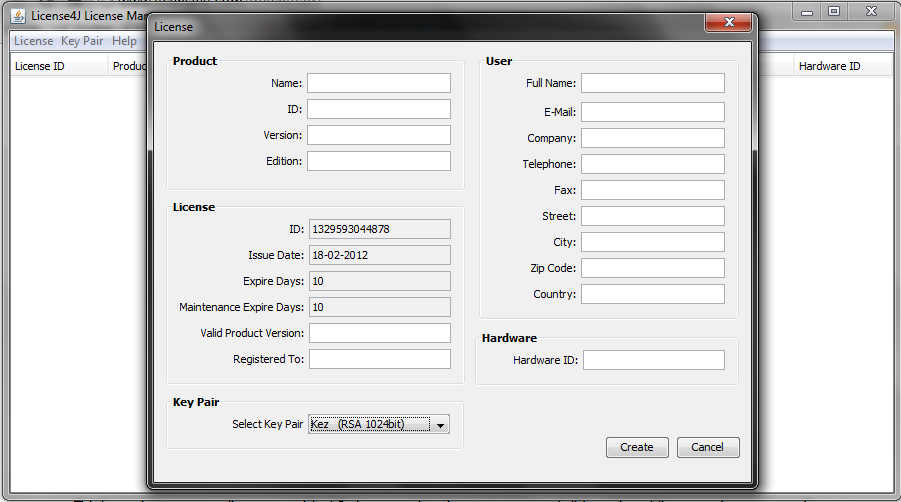
\includegraphics[width=12cm]{figures/license4j.PNG}
\caption{License4j UI pro tvorbu licencí}
\label{fig:license4j-ui} 
\end{center}
\end{figure}

\subsection*{Vlastnosti}
Aplikace je dostupná volně ke stažení, verze zdarma umožňuje vytvářet licence s
platností 10 dní, licenci pro plnou funkčnost je možné zakoupit za částku \$35.
K produktu je navíc možné dokoupit roční rozšířenou podporu za \$15.

Distribuovaná verze obsahuje knihovny a GUI bez zdrojových kódů. Mezi vlastnosti
produktu patří:

\begin{itemize}
  \item Ruční výroba licenčního souboru pomocí dodané aplikace s GUI,
  předdefinované položky v licenci
  \item Možnost zabudování MAC adresy nebo hostname do licenčního souboru
  \item Kontrola platnosti licence za běhu pomocí veřejného klíče 
\end{itemize}

\subsection*{Zhodnocení}
License4j je jendoduchoá knihovna s velmi omezeným použitím, čemuž odpovídá i
poměrně nízká pořizovací cena. 

Výhodou může být snadná integrovatelnost s existujícími aplikacemi a snadná
výroba licenčních klíčů pomocí dodaného GUI.

Hlavní nevýhodou tohoto produktu je potřeba ručně generovat licenční soubory
pro každého zákazníka, což může být při distribuci většího množství licencí
problematické. Licence je sice možné vázat na MAC adresu nebo hostname, to ale
není pro reálné použití příliš vhodné.


\section{JLicense}
Podobně jako u předchozího produktu se v případě JLicense\cite{jlicense} jedná o
jednoduchou knihovnu, která umožňuje pomocí GUI generovat licenční klíče,
jejichž platnost se poté v aplikaci kontroluje pomocí digitálního podpisu.

\begin{figure}[H]
\begin{center}
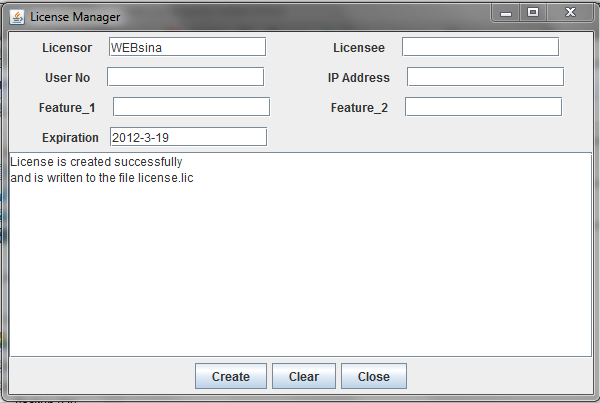
\includegraphics[width=12cm]{figures/jlicense.PNG}
\caption{JLicense UI pro tvorbu licencí}
\label{fig:jlicense-ui} 
\end{center}
\end{figure}

\subsection*{Vlastnosti}
Knihovnu je možné stáhnout a používat zdarma. V případě zájmu je možné koupit
zdrojové kódy za cenu \$50. Vlastnosi produktu jsou:

\begin{itemize}
  \item Ruční výroba licenčního souboru pomocí dodané aplikace s GUI,
  předdefinované položky v licenci
  \item Možnost zabudování IP adresy do licence
\end{itemize}

\subsection*{Zhodnocení}
Jedná se o produkt funkčně shodný s knihovnou License4j. Výhodou může být
možnost neomezeného použití zdarma a také dostupnost zdrojových kódů za
poplatek.


\section{Rampart}
Posledním ze zástupců kategorie malých knihoven je knihovna
Rampart\cite{rampart}. Stejně jako v předchozích připadech se produkt skládá z
GUI pro generování licenčních souborů a runtime knihovny pro ověřování
vygenerovaných licencí.

\begin{figure}[H]
\begin{center}
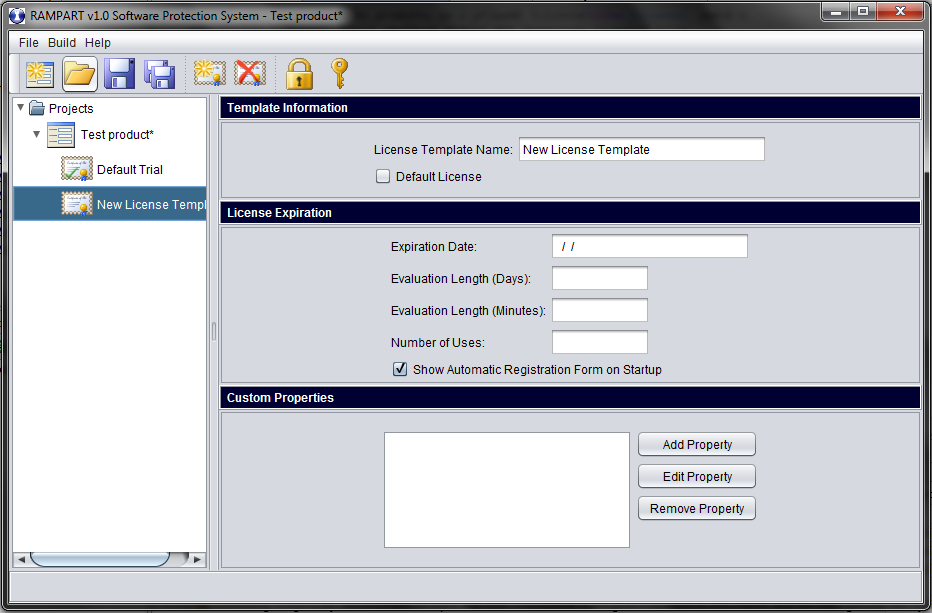
\includegraphics[width=12cm]{figures/rampart.PNG}
\caption{Rampart UI pro tvorbu licencí}
\label{fig:rampart-ui} 
\end{center}
\end{figure}

\subsection*{Vlastnosti}
Trial verzi s omezenou platností na 30 dní je možné zdarma stáhnout z webových
stránek výrobce, licenci na plnou verzi je možné zakoupit za \$29. Mezi
vlastnosti produktu patří:

\begin{itemize}
  \item Výroba a správa licencí pomocí GUI
  \item Podpora pro trial verze
\end{itemize}

\subsection*{Zhodnocení}
Výhodou tohoto produktu oproti předchozím je mnohem propracovanější nástroj pro
správu licencí. Runtime knihovna také umožňuje zobrazovat dialogy usnadňující
získání licence.

nevýhodou může být fakt, že vydané licence není možné jakkoliv vázat na
hardware.

\section{Protection! 4}

Produkt Protection! 4\cite{protection} je první ze zkoumaných produktů přímo
určený pro nasazení v enterprise prostředí. Obsahuje jak velmi pokročilý nástroj
umožňující vytváření, správu a integraci licencí, tak i server pro centrální
správu licencí.

\begin{figure}[H]
\begin{center}
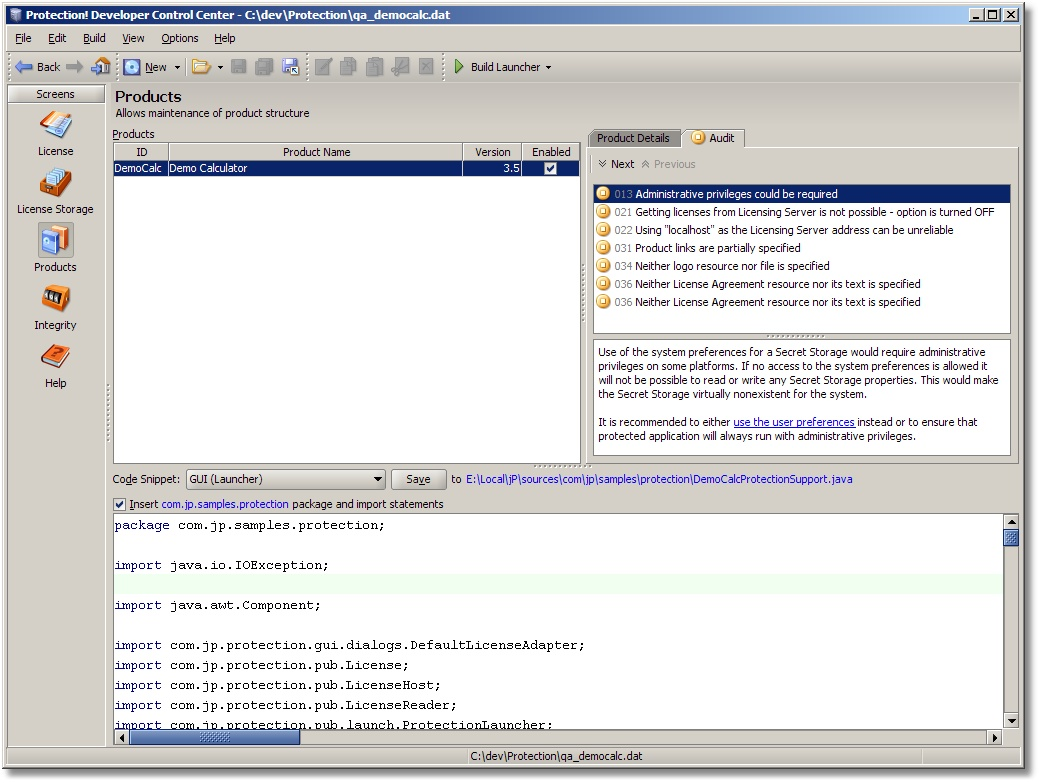
\includegraphics[width=12cm]{figures/protection4.PNG}
\caption{Protection developer control center}
\label{fig:protection4-ui} 
\end{center}
\end{figure}

\subsection*{Vlastnosti}
Jendá se o ryze komerční řešení, ze stránek výrobce se dají stáhnout všechny
potřebné nástroje, je ale potřeba kontaktovat výrobce ohledně vystavení trial
licence. Cena je \$997 za licenci pro desktopovou aplikaci pro jednoho
vývojáře, serverový backend stojí \$5000 na rok na jedno procesorové jádro. Je
možné také dokoupit dodatečnou podporu.

\begin{itemize}
  \item Výroba a správa licencí pomocí pokročilého grafického nástroje
  \item Grafický nástroj usnadňující integracio ochrany do aplikace vytvářející
  vlastní launcher
  \item Podpora pro trial verze
  \item Webová služba umožňující integraci s existujícími systémy
  \item Možnost vázat licenci na hardware počítače
  \item Licenční server včetně webového rozhraní pro správu licencí
  \item Možnost vydávat licence vázané na hardware i licence omezené počtem
  souběžně běžících kopií
  \item Kontrola integrity aplikace pro znesnadnění odstranění ochrany
\end{itemize}

\subsection*{Zhodnocení}
Jedná se o pokročilé řešení určené pro větší podniky s velkým množstvím
vlastností. Nevýhodou může být vysoká pořizovací cena pro menší projekty.

\section{LM-X License Manager}
LM-X License Manager\cite{lm-x} je další z komerčních licenčních nástrojů
orientovaný na velké společnosti. Produkt je distribuován v podobě SDK napsaného
v C++, pro integraci s aplikacemi napsanými v Javě výrobce poskytuje obalovací
třídy.

\subsection*{Vlastnosti}
Výrobce umožňuje stažení testovací verze s omezenou dobou platnosti zdarma po
vyplnění kontaktního formuláře. Platnost testovací verze je možné prodloužit za
poplatek \EUR{200} na 3 měsíce. Cena licence pro komerční použití závisí na
obratu společnosti a počtu platforem. Nejlevnější licence pro společnost s
obratem pod \EUR{1M} vyjde na \EUR{1500} za rok a \EUR{550} za každou další
platformu.

Vlastnosti produktu:

\begin{itemize}
  \item Integrace s aplikacemi pomocí výrobcem dodaného SDK
  \item Možnost vystavovat licence vázané na hardware i plovoucí licence
  \item Licenční server pro centrální správu licencí 
\end{itemize}

\subsection*{Zhodnocení}
Opět se jedná o profesionální licenční řešení, takže jeho hlavní výhodou je
velké množství funkcí a podpora od výrobce.

Jako nevýhoda se kromě ceny může také jevit skutečnost, že dodávaná knihovna je
napsaná v C++ a pro použití s aplikacemi napsanými v Javě je potřeba používat
obalovací třídy. K aplikaci je tedy nutné přibalit i zkompilované knihovny pro
každou podporovanou platformu.

\section{Vyhodnocení}
Výsledky zkoumaných řešení jsou shrnuty v následující tabulce:

\begin{table}\centering
	\caption[Results]{Porovnání hodnocených produktů}\label{tab:research-results}
	\begin{tabular}{|l|l|l|l|}\hline
		Název			& Podporované platformy	& Podpora Eclispe/OSGi	& Cena
		\tabularnewline \hline \hline 
		License4j		& Java					& Ne					& \$35		
		\tabularnewline \hline
		JLicense		& Java					& Ne					& Zdarma, \$50 za zdrojov0 kódy
		\tabularnewline \hline
		Rampart			& Java					& Ne					& \$29
		\tabularnewline \hline
		Protection! 4	& Java					& Ne					& \$997 za vývojáře, \$5000 za serverovou
		část na rok 
		\tabularnewline \hline
		LM-X License Manager & Windows, Linux, MacOS, AIX, Solarix,\ldots & Ne & Dle
		obratu firmy, minim8ln2 \EUR{1500} na rok + \EUR{550} za platformu
		\tabularnewline \hline
	\end{tabular}
\end{table}

Průzkum ukazuje, že dostupná řešení se dělí ve své podstatě na 2 kategorie:

\begin{itemize}
  \item Malé knihovny – poskytují pouze základní funkcionalitu v podobě
  vytváření licencí pomocí dodaného nástroje a knihovnu pro ověřování platnosti
  licence za běhu licencované aplikace. V případě, že nehledáme příliš
  sofistikované řešení může být jejich použití vhodné, obzvláště pak s
  přihlédnutím k ceně. Ta se pohybuje v rozmezí několika desítek dolarů.
  \item Komerční řešení – produkty určené k použití v enterprise prostředí.
  Vynikají především množstvím poskytované funkcionality – od vystavování trial
  licencí, přes licence vázané na hardware až po serverová řešení pro distribuci
  licencí. Tomu ovšem také odpovídá cena, která se pohybuje v řádu tísíců
  dolarů, často s nutností připlácet za další vývojáře, platformy a také za
  každoroční obnovení licence.
\end{itemize}

Ukazuje se také, že žádný z dostupných nástrojů neobsahuje podporu pro aplikace
psané na platformě Eclipse, případně OSGi.
% License4J - http://www.license4j.com/
% - v podstate jen podepsani licencnich udaju + GUI
% - cena = $35
% - generovani HW otisku
%   - mac 
%   - hostname
% - licence se generuje pomoci swingove aplikace
% - do aplikace se zabudujuje verejny klic, overuje se licence
% 
% 
% jProductivity Protection!
% - cena $997 per developer and backend $5,000 per year; per CPU 
% - server + klient reseni
% 
% JLicense - http://www.websina.com/products/jlicense.html#
% - podobne jako License4J
% - cena = $50
% - IP adressa, MAC adresa, User number
% 
% http://www.jproductivity.com/products/protection/protection.htm
% 
% Rampart
% - vytvoreni podepsaneho licencniho souboru, ktery se kontroluje
% - neumoznuje vazbu na HW
% - cena $29


%LM-X
%- 1500



%%%%%%%%%%%%%%%%%%%%%%%%%%%%%%%%%%%%%%%%%%%%%
% Kapitola 3 - Analýza
\chapter{Analýza}

V této kapitole je provedena analýza požadavků a je navržena architektura
výsledné aplikace.



\section{Požadavky}

\subsection{Nefunkční požadavky}

Výsledný navrhovaný nástroj musí splňovat následující podmínky

\subsubsection*{Implementace v jazyce Java}

Vzhledem k tomu, že důvodem ke vzniku práce bylo dodání licencovacího mechanismu
do existujících aplikací napsaných v jazyce Java, jedním z hlavních požadavků
je celý navržený systém implementovat v Javě. Ačkoliv Java umožňuje využívat
knihovny napsané například v C/C++ pomocí JNI\cite{jni} nebo JNA\cite{jna}, je
použití nativních knihoven mnohem snadnější.


\subsubsection*{Podpora pro aplikace napsané na platformě Eclipse RCP}

Důvodem tohoto požadavku je fakt, že existující aplikace jsou napsány právě na
platformě Eclipse RCP\cite{eclipse-rcp}. Pro snadnější integraci by měla být
klientská část navrhovaného systému distribuovaná v podobě pluginu.

Důsledkem tohoto požadavku je kromě podoby výsledné distribuce klientské části
také omezení týkající se knihoven třetích stran. Využívany by měli být především
takové knihovny, které jsou obvykle obsaženy ve většině distribucí aplikací
napsaných na platformě Eclipse RCP. Například v případě použití GUI by měla být
použita knihovna SWT\cite{swt}.

\subsubsection*{Funkčnost na operačních systémech Windows a Linux}

Tento požadavek opět souvisí s tím, že existující aplikace podporují právě tyto
operační systémy. Navíc jsou systémy Windows a Linux nejsnáze dostupné pro
testovací účely. 

Ačkoliv je Java multiplatformní jazyk, možnosti týkající se zístkávání informací
specifických pro konkrétní operační systém jsou značně omezené. Pokud chceme
vázat licenci na konkrétní hardware, je zapotřebí mnohem těsnější vazby s
operačním systémem, než jakou Java umožňuje. Z tohoto důvodu bude nutné část
funkcionality přizpůsobit konkrétnímu operačnímu systému a tuto část
implementovat pro všechny podporované platformy. Jako cílové byly zvoleny
operační systémy Windows a Linux, mělo by ale být možné v případě potřeby snadno
rozšířit podporu i pro další operační systémy.


\subsubsection*{Snadná integrovatelnost do již existujících aplikací}
 
K rozhodnutí o přidání funkčnosti pro licencování do aplikace může dojít až v
pozdější fázi vývoje, případně může být požadavek licencování přidat do již
hotového produktu. Z tohoto důvodu by měla být integrace co nejjednodušší.
Modulární architektura platformy Eclipse RCP toto v případě integrace do
desktopové aplikace usnadní. Stejný požadavek ale můžemem mít také na serverové
straně. Pokud již máme existující databázi uživatelů, mohli bychom ji chtít
využít pro vystavení licencí.
  
\subsubsection*{Centrální správa licencí}

Aby bylo možné mít přehled o všech vydaných licencích, je nutné licence
spravovat centrálně.

\subsubsection*{Webové GUI pro snadnějš správu licencí}

Protože o vydávání licencí se běžně stará obchodní oddělení, je potřeba
vytvořit grafické uživatelské rozhraní, které umožní uživatelům spravovat vydané
licence. Z hlediska snadnosti použití a platformní nezávislosti se jako
nejvhodnější jeví webové rozhraní.


\subsection{Funkční požadavky}

\subsubsection*{Vlastnosti licence}

Licence vydávané a ověřované implementovaným licenčním nástrojem musí mít
následující vlastnosti.

\begin{itemize}
  \item Časové omezení – počátek nebo konec platnosti licence je možné časově
  omezit
  \item Vazba na hardware – platnost licence je možné vázat na konkrétní
  hardware
  \item Licencované vlastnosti - do vystavené licence je možné zanást
  informace o povolených vlastnostech licencovaného produktu.
\end{itemize}

\subsubsection*{Vlastnosti klientské části}

Tyto vlastnosti bude mít klientská část licenčního mechanismu, která se bude
zabudovávat do aplikace.

\begin{itemize}
  \item Online kontrola platnosti – platnost licence bude je ověřit proti
  licenčnímu serveru.
  \item Offline kontrola platnosti – platnost údajů uvedených v licenci je
  možné ověřit bez nutnosti připojení k centrálnímu serveru. Jedná se především
  o kontrolu dat počátku a konce platnosti a kontroly vazby na hardware.
\end{itemize}

\subsubsection*{Vlastnosti serverové části}

\begin{itemize}
  \item Zobrazení přehledu vystavených licencí
  \item Vytvoření nové licence
  \item Zneplatnění licence
  \item Ověření platnosti vydané licence
\end{itemize}

\section{Architektura}

Jako nejvhodnější architektura pro navrhovaný produkt je typ klient-server.
Rozvržení jednotlivých komponent je zobrazeno v diagramu na obrázku
\ref{fig:deployment}.

\begin{figure}[H]
\begin{center}
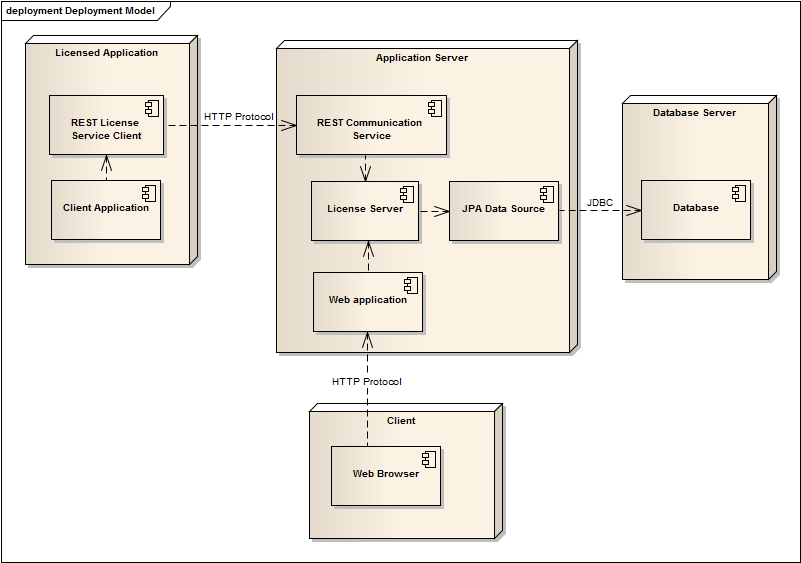
\includegraphics[width=12cm]{figures/deployment.png}
\caption{Diagram nasazení jednotlivých komponent}
\label{fig:deployment} 
\end{center}
\end{figure}

\subsection{Serverová část}

Účelem serverové části je poskytovat informace o vydaných licencích a ověřovat
jejich platnost. Serverová část může být integrována do existující serverové
aplikace, nebo nasazena jako samostatná aplikace. Komponenty serverové aplikace
jsou na obrázku \ref{fig:components-server}.


\begin{figure}[H]
\begin{center}
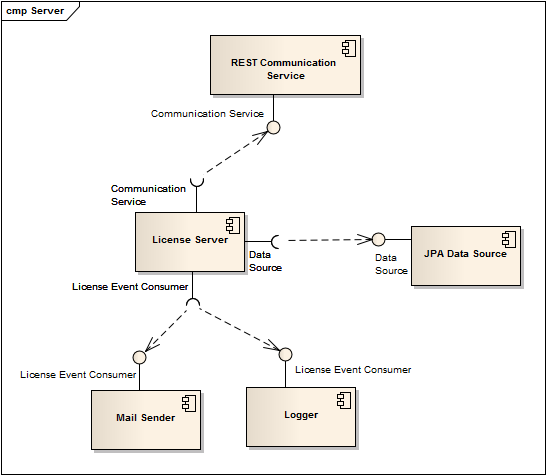
\includegraphics[width=12cm]{figures/components-server.png}
\caption{Diagram komponent serverové části}
\label{fig:components-server} 
\end{center}
\end{figure}

Pro zajištění rozšiřitelnosti, snadné integrace do existujících aplikací a dobré
testovatelnosti je část funkcionality serverové části rozdělena do několika
komponent s definovaným rozhraním.

\subsubsection*{License Server}

Hlavní část serverové aplikace obsahující logiku spojenou s ověřováním
licencí. Jejím úkolem je odpovídat na požadavky od klientských aplikací na
ověření platnosti licence uložené v databázi. Jendotlivé části zajišťující
komunikaci s klienty a databází jsou dekomponovány do samostatných částí a
komunikace s nimi probíhá pomocí pevně daného rozhraní. To umožňuje udržet
komponentu nezávislou na použitém komunikačním protokolu a databázové vrstvě.

\subsubsection*{Communication Service}

Communication Service je komponenta odpovědná za komunikaci s klientskými
aplikacemi. Jejím vyčleněním do samostatné části je dosaženo odstranění
závislosti na použitém protokolu pro komunikaci s klientskými aplikacemi.
Komponenta Communication Service překládá požadavky na ověření platnosti licence
z podoby specifické pro použitý komunikační protokol (XML, JSON, Serialozované
objekty, \ldots) do univerzální podoby akceptované částí License Server.

V implementační části bude tato komponenta naimplementována v podobě
RESTful\cite{rest} webové služby.

\subsubsection*{Data Source}

Komponenta Data Source slouží k načítání a ukládání informací o vydaných
licencích do persistentního úložiště. Poskytuje serverové aplikaci základní operace jako
nalezení licence podle identifikátoru a zaznamenání aktivace licence.  




\begin{conclusion}

\end{conclusion}

\bibliographystyle{iso690.bst}
\bibliography{ref}

\appendix

\printglossaries



\end{document}
